\section{Softwarearchitektur und Design}

\begin{concept}{Überblick Software Development}\\
Die Entwicklung von Software erfolgt in verschiedenen Ebenen:
\begin{itemize}
    \item Business Analyse \& Domänenmodell: Requirements
    \item Architektur: Logische Struktur des Systems
    \item Design: Detaillierte Systemspezifikation
    \item Entwicklung: Konkrete Umsetzung
\end{itemize}

Architektur und Design sind eng verzahnt und bauen aufeinander auf:
\begin{itemize}
    \item Architektur definiert das "große Ganze"
    \item Design spezifiziert die Details der Umsetzung
    \item Beides basiert auf Requirements und führt zur Implementation
\end{itemize}
%todo: better resolution image
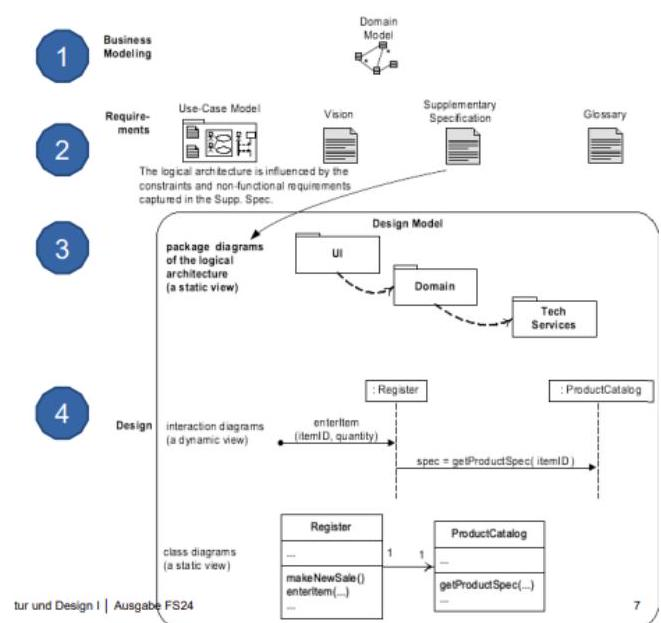
\includegraphics[width=\linewidth]{images/2024_12_29_0d1d7b5551ea1b4b41bdg-07(2)}
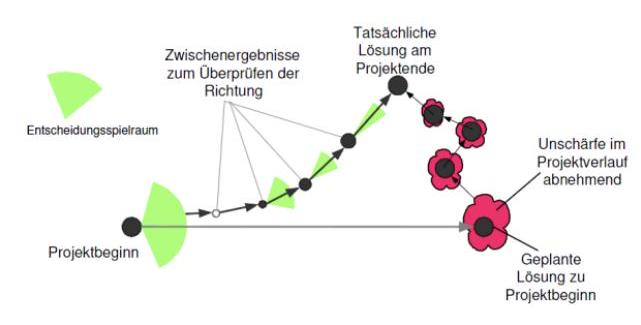
\includegraphics[width=\linewidth]{images/2024_12_29_0d1d7b5551ea1b4b41bdg-08(1)}
\end{concept}




\columnbreak

\subsubsection{Architektur}

\begin{definition}{Software-Architektur}\\
Die Gesamtheit der wichtigen Entwurfs-Entscheidungen:
\begin{itemize}
    \item Grundlegende Strukturen und Komponenten
    \item Beziehungen zwischen Komponenten und zur Umgebung
    \item Heutige und zukünftige Anforderungen
    \item Leitende Prinzipien und Patterns
    \item Erfüllung der Qualitätsanforderungen
    \item Weiterentwicklungsmöglichkeiten
\end{itemize}

Ziele der Architektur:
\begin{itemize}
    \item Erfüllung aktueller und zukünftiger Anforderungen
    \item Ermöglichung von Weiterentwicklung
    \item Sicherstellung von Qualitätsattributen
    \item Reduktion von technischen Risiken
\end{itemize}
\end{definition}

\begin{concept}{Von Requirements zur Architektur}\\
Die Architektur wird systematisch aus den Anforderungen abgeleitet:

\textbf{Analyse der Anforderungen:}
\begin{itemize}
    \item Funktionale Anforderungen
    \item Nicht-funktionale Anforderungen (Qualitätsattribute)
    \item Randbedingungen
    \item Stakeholder-Bedürfnisse
\end{itemize}

\textbf{Architektur-Entscheidungen:}
\begin{itemize}
    \item Auswahl von Architekturstilen
    \item Definition von Komponenten
    \item Festlegung von Schnittstellen
    \item Bewertung von Alternativen
\end{itemize}
\end{concept}

\begin{theorem}{Architekturanalyse}\\
Die Analyse erfolgt iterativ mit den Anforderungen:
\begin{itemize}
    \item Analyse funktionaler und nicht-funktionaler Anforderungen
    \item Abstimmung mit Stakeholdern
    \item Kontinuierliche Weiterentwicklung
\end{itemize}
%todo: better resolution image
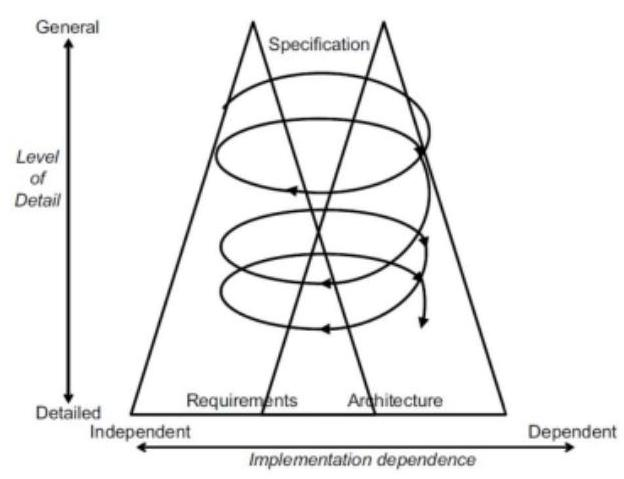
\includegraphics[width=0.9\linewidth]{images/2024_12_29_0d1d7b5551ea1b4b41bdg-08}
\end{theorem}

\begin{corollary}{ISO 25010 und FURPS+}\\
\textbf{ISO 25010:}
Hierarchisches Qualitätsmodell mit:
\begin{itemize}
    \item Hauptcharakteristiken
    \item Subcharakteristiken
    \item Messbare Metriken
    \item Präzise Anforderungsformulierung
\end{itemize}

\textbf{FURPS+:}
\begin{itemize}
    \item Functionality (Funktionalität)
    \item Usability (Benutzbarkeit)
    \item Reliability (Zuverlässigkeit)
    \item Performance (Leistung)
    \item Supportability (Wartbarkeit)
    \item + (Implementation, Interface, Operations, Packaging, Legal)
\end{itemize}

Die Analyse dieser Qualitätsattribute ist zentral für Architekturentscheidungen.
\end{corollary}


\subsection{Modulkonzept und Architekturmuster}

\begin{concept}{Modulkonzept}\\
Ein Modul (Baustein, Komponente) ist eine logisch zusammengehörige Einheit:

\textbf{Eigenschaften:}
\begin{itemize}
    \item Möglichst autarkes Teilsystem
    \item Minimale externe Schnittstellen
    \item Enthält alle benötigten Funktionen/Daten
    \item Kann sein: Paket, Library, Service, Komponente
\end{itemize}

\textbf{Qualitätskriterien:}
\begin{itemize}
    \item \textbf{Kohäsion:} Stärke des inneren Zusammenhangs
    \item \textbf{Kopplung:} Grad der Abhängigkeit zu anderen Modulen
\end{itemize}
\end{concept}

\begin{definition}{Schnittstellen (Interfaces)}\\
Ein Modul definiert seine Interaktion über Schnittstellen:

\textbf{Exportierte Schnittstellen:}
\begin{itemize}
    \item Definieren angebotene Funktionalität
    \item Garantierter Vertrag nach außen
    \item Einzige externe Sichtbarkeit
\end{itemize}

\textbf{Importierte Schnittstellen:}
\begin{itemize}
    \item Verwendung anderer Module
    \item Definierte Abhängigkeiten
    \item Basis für Kopplung
\end{itemize}
\end{definition}

\begin{theorem}{Architekturprinzipien}\\
Grundlegende Prinzipien für gute Architektur:

\textbf{Separation of Concerns:}
\begin{itemize}
    \item Trennung von Verantwortlichkeiten
    \item Klare Modulgrenzen
    \item Reduzierte Komplexität
\end{itemize}

\textbf{Information Hiding:}
\begin{itemize}
    \item Kapselung von Implementierungsdetails
    \item Definierte Schnittstellen
    \item Änderbarkeit ohne Seiteneffekte
\end{itemize}

\textbf{Loose Coupling:}
\begin{itemize}
    \item Minimale Abhängigkeiten
    \item Austauschbarkeit
    \item Unabhängige Entwicklung
\end{itemize}
\end{theorem}

\begin{concept}{Architekturmuster Übersicht}\\
Bewährte Lösungsmuster für wiederkehrende Architekturprobleme:

\textbf{Grundlegende Muster:}
\begin{itemize}
    \item \textbf{Layered Pattern:} Schichtenarchitektur
    \item \textbf{Client-Server Pattern:} Verteilte Dienste
    \item \textbf{Master-Slave Pattern:} Verteilte Verarbeitung
    \item \textbf{Pipe-Filter Pattern:} Datenstromverarbeitung
    \item \textbf{Broker Pattern:} Vermittler zwischen Endpunkten
    \item \textbf{Event-Bus Pattern:} Nachrichtenverteilung
    \item \textbf{MVC Pattern:} Trennung von Daten und Darstellung
\end{itemize}

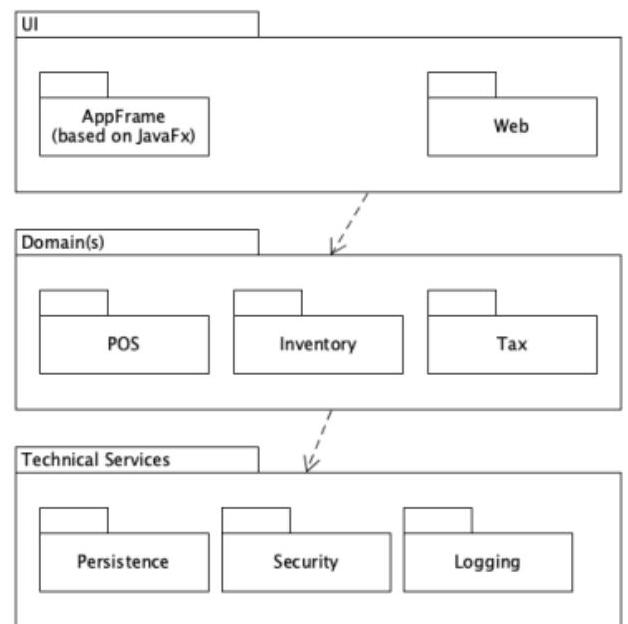
\includegraphics[width=0.9\linewidth]{images/2024_12_29_0d1d7b5551ea1b4b41bdg-09(1)}
\end{concept}

\begin{KR}{Clean Architecture}\\
Prinzipien nach Robert C. Martin:

\textbf{Hauptprinzipien:}
\begin{itemize}
    \item Unabhängigkeit von Frameworks
    \item Testbare Business Rules
    \item Unabhängigkeit von UI
    \item Unabhängigkeit von Datenbank
    \item Unabhängigkeit von externen Systemen
\end{itemize}

\textbf{Schichten (von innen nach außen):}
\begin{enumerate}
    \item Entities (Enterprise Business Rules)
    \item Use Cases (Application Business Rules)
    \item Interface Adapters (Controllers, Presenters)
    \item Frameworks \& Drivers (UI, DB, Devices)
\end{enumerate}

\textbf{Dependency Rule:}
Abhängigkeiten dürfen nur nach innen zeigen.
\end{KR}

\begin{example2}{Clean Architecture Implementation}\\
\begin{lstlisting}[language=Java, style=base]
// Enterprise Business Rules (Entity)
public class Order {
    private List<OrderItem> items;
    
    public Money calculateTotal() {
        return items.stream()
                   .map(OrderItem::getSubtotal)
                   .reduce(Money.ZERO, Money::add);
    }
}

// Application Business Rules (Use Case)
public class CreateOrderUseCase {
    private OrderRepository repository;
    
    public OrderId execute(CreateOrderCommand cmd) {
        Order order = new Order(cmd.getItems());
        validateOrder(order);
        return repository.save(order);
    }
}

// Interface Adapters
public class OrderController {
    private CreateOrderUseCase useCase;
    
    public OrderResponse createOrder(OrderRequest req) {
        CreateOrderCommand cmd = mapToCommand(req);
        OrderId id = useCase.execute(cmd);
        return new OrderResponse(id);
    }
}
\end{lstlisting}
\end{example2}

\begin{concept}{Modulkonzept}\\
Ein Modul (Baustein, Komponente) wird bewertet nach:
\begin{itemize}
    \item \textbf{Kohäsion:} Innerer Zusammenhang
    \item \textbf{Kopplung:} Externe Abhängigkeiten
\end{itemize}

\textbf{Eigenschaften:}
\begin{itemize}
    \item Autarkes Teilsystem
    \item Minimale externe Schnittstellen
    \item Enthält alle benötigten Funktionen/Daten
    \item Verschiedene Formen: Paket, Library, Service
\end{itemize}
\end{concept}

\begin{concept}{Architektursichten}\\
Das N+1 View Model beschreibt verschiedene Perspektiven:\\
%todo: better resolution image
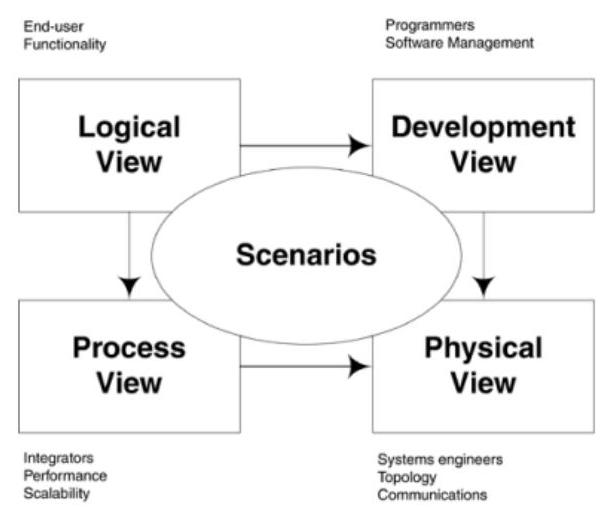
\includegraphics[width=0.9\linewidth]{images/2024_12_29_0d1d7b5551ea1b4b41bdg-09}
\end{concept}

\begin{theorem}{Qalitätskriterien}\\
Grundlegende Strategien zur Erfüllung von Qualitätsanforderungen:

\textbf{Performance:}
\begin{itemize}
    \item Resource Pooling
    \item Caching
    \item Parallelisierung
    \item Lazy Loading/Evaluation
\end{itemize}

\textbf{Verfügbarkeit:}
\begin{itemize}
    \item Redundanz
    \item Health Monitoring
    \item Failover Mechanismen
    \item Circuit Breaker
\end{itemize}

\textbf{Wartbarkeit:}
\begin{itemize}
    \item Separation of Concerns
    \item Information Hiding
    \item Interface-basierte Kommunikation
    \item Standardisierung
\end{itemize}

\begin{itemize}
    \item \textbf{Modularität:}
    \begin{itemize}
        \item Klare Modulgrenze
        \item Minimale Abhängigkeiten
        \item Hohe Kohäsion
    \end{itemize}
    
    \item \textbf{Testbarkeit:}
    \begin{itemize}
        \item Isolation von Komponenten
        \item Mockbarkeit von Abhängigkeiten
        \item Testautomatisierung
    \end{itemize}
    
    \item \textbf{Änderbarkeit:}
    \begin{itemize}
        \item Lokalisierung von Änderungen
        \item Erweiterbarkeit
        \item Backward Compatibility
    \end{itemize}

    \item \textbf{Erweiterbarkeit:}
    \begin{itemize}
        \item Offene Schnittstellen
        \item Plugin-Systeme
        \item Service-Orientierung
    \end{itemize}
\end{itemize}
\end{theorem}

\subsubsection{Architektur-Taktiken und Best Practices}

\begin{KR}{Architekturentwurf}\\
Systematischer Ansatz für Architekturentscheidungen:
\begin{enumerate}
    \item \textbf{Anforderungen analysieren}
    \begin{itemize}
        \item Funktionale Anforderungen gruppieren
        \item Nicht-funktionale Anforderungen priorisieren
        \item Randbedingungen identifizieren
    \end{itemize}
    
    \item \textbf{Einflussfaktoren bewerten}
    \begin{itemize}
        \item Technische Faktoren
        \item Organisatorische Faktoren
        \item Wirtschaftliche Faktoren
    \end{itemize}
    
    \item \textbf{Alternativen evaluieren}
    \begin{itemize}
        \item Vor- und Nachteile abwägen
        \item Proof of Concepts durchführen
        \item Risiken analysieren
    \end{itemize}
    
    \item \textbf{Entscheidung dokumentieren}
    \begin{itemize}
        \item Begründung festhalten
        \item Verworfene Alternativen dokumentieren
        \item Annahmen dokumentieren
    \end{itemize}
\end{enumerate}
\end{KR}

\begin{KR}{Architekturentwurf}\\
\textbf{Schritte:}
\begin{enumerate}
    \item Anforderungen analysieren
    \item Architekturstil wählen
    \item Module identifizieren
    \item Schnittstellen definieren
    \item Mit Stakeholdern abstimmen
\end{enumerate}

\textbf{Qualitätskriterien:}
\begin{itemize}
    \item Änderbarkeit
    \item Wartbarkeit
    \item Erweiterbarkeit
    \item Testbarkeit
\end{itemize}
\end{KR}

\begin{example2}{Architekturentwurf}\\
\textbf{Aufgabe:} Entwerfen Sie die grundlegende Architektur für ein Online-Banking-System.

\textbf{Lösung:}
\begin{itemize}
    \item \textbf{Anforderungsanalyse:}
    \begin{itemize}
        \item Sicherheit (ISO 25010)
        \item Performance (FURPS+)
        \item Skalierbarkeit
    \end{itemize}
    
    \item \textbf{Architekturentscheidungen:}
    \begin{itemize}
        \item Mehrschichtige Architektur
        \item Microservices für Skalierbarkeit
        \item Sicherheitsschicht
    \end{itemize}
    
    \item \textbf{Module:}
    \begin{itemize}
        \item Authentifizierung
        \item Transaktionen
        \item Kontoführung
    \end{itemize}
\end{itemize}
\end{example2}

\begin{example2}{Typische Prüfungsaufgabe: Architekturanalyse}\\
\textbf{Aufgabenstellung:}
Analysieren Sie folgende Anforderungen und leiten Sie architektonische Konsequenzen ab:
\begin{itemize}
    \item System muss 24/7 verfügbar sein
    \item 10.000 gleichzeitige Benutzer
    \item Reaktionszeit unter 1 Sekunde
    \item Jährliche Wartungsfenster maximal 4 Stunden
\end{itemize}

\textbf{Lösung:}
\begin{itemize}
    \item \textbf{Architekturentscheidungen:}
    \begin{itemize}
        \item Verteilte Architektur für Hochverfügbarkeit
        \item Load Balancing für gleichzeitige Benutzer
        \item Caching-Strategien für Performanz
        \item Blue-Green Deployment für Wartung
    \end{itemize}
    
    \item \textbf{Begründungen:}
    \begin{itemize}
        \item Verteilung minimiert Single Points of Failure
        \item Load Balancer verteilt Last gleichmäßig
        \item Caching reduziert Datenbankzugriffe
        \item Blue-Green erlaubt Updates ohne Downtime
    \end{itemize}
\end{itemize}
\end{example2}



\begin{KR}{Architektur-Review durchführen}\\
\textbf{Vorgehen:}
\begin{enumerate}
    \item \textbf{Vorbereitung}
    \begin{itemize}
        \item Architektur-Dokumentation zusammenstellen
        \item Review-Team zusammenstellen
        \item Checklisten vorbereiten
    \end{itemize}
    
    \item \textbf{Durchführung}
    \begin{itemize}
        \item Architektur vorstellen
        \item Anforderungen prüfen
        \item Entscheidungen hinterfragen
        \item Risiken identifizieren
    \end{itemize}
    
    \item \textbf{Nachbereitung}
    \begin{itemize}
        \item Findings dokumentieren
        \item Maßnahmen definieren
        \item Follow-up planen
    \end{itemize}
\end{enumerate}

\textbf{Prüfkriterien:}
\begin{itemize}
    \item Anforderungserfüllung
    \item Technische Machbarkeit
    \item Zukunftssicherheit
    \item Best Practices
\end{itemize}
\end{KR}

\begin{KR}{Architektur-Review}\\
Systematische Überprüfung der Architektur:

\textbf{1. Vorbereitung}
\begin{itemize}
    \item Architektur-Dokumentation sichten
    \item Qualitätsanforderungen prüfen
    \item Review-Team zusammenstellen
    \item Checklisten erstellen
\end{itemize}

\textbf{2. Durchführung}
\begin{itemize}
    \item Architektur-Walkthrough
    \item Szenario-basierte Evaluation
    \item Risiko-Analyse
    \item Trade-off Analyse
\end{itemize}

\textbf{3. Nachbereitung}
\begin{itemize}
    \item Ergebnisse dokumentieren
    \item Maßnahmen ableiten
    \item Priorisierung vornehmen
    \item Follow-up planen
\end{itemize}
\end{KR}

\begin{example2}{Architektur-Review}\\

\begin{lstlisting}[language=Java, style=basesmol]
// Beispiel fuer gute Testbarkeit
public class OrderService {
    private final OrderRepository repository;
    private final PaymentGateway paymentGateway;
    
    // Dependency Injection ermoeglicht einfaches Mocking
    public OrderService(
            OrderRepository repository,
            PaymentGateway paymentGateway) {
        this.repository = repository;
        this.paymentGateway = paymentGateway;
    }
    
    // Klare Methoden-Verantwortlichkeiten
    public OrderResult createOrder(OrderRequest request) {
        validateRequest(request);
        Order order = createOrderEntity(request);
        PaymentResult payment = processPayment(order);
        return createOrderResult(order, payment);
    }
}
\end{lstlisting}
\end{example2}

\begin{KR}{Architektur-Evaluation}\\
Systematische Bewertung einer Softwarearchitektur:

\textbf{1. Qualitätsattribute identifizieren}
\begin{itemize}
    \item Performance
    \item Skalierbarkeit
    \item Wartbarkeit
    \item Sicherheit
\end{itemize}

\textbf{2. Szenarien entwickeln}
\begin{itemize}
    \item Normale Nutzung
    \item Grenzfälle
    \item Fehlerfälle
    \item Wartungsszenarien
\end{itemize}

\textbf{3. Architektur analysieren}
\begin{itemize}
    \item Strukturanalyse
    \item Verhaltensanalyse
    \item Trade-off Analyse
\end{itemize}

\textbf{4. Risiken identifizieren}
\begin{itemize}
    \item Technische Risiken
    \item Geschäftsrisiken
    \item Architekturrisiken
\end{itemize}
\end{KR}




\raggedcolumns
\pagebreak

\subsection{Design Patterns und UML-Modellierung}

\begin{concept}{Statische vs. Dynamische Modelle}\\
UML bietet verschiedene Diagrammtypen für unterschiedliche Aspekte:

\textbf{Statische Modelle:}
\begin{itemize}
    \item Fokus auf Struktur und Beziehungen
    \item UML-Klassendiagramm für Klassen, Attribute, Methoden
    \item UML-Paketdiagramm für Modularisierung
    \item UML-Komponentendiagramm für Systembausteine
    \item UML-Verteilungsdiagramm für Deployment
\end{itemize}

\textbf{Dynamische Modelle:}
\begin{itemize}
    \item Fokus auf Verhalten und Interaktion
    \item UML-Sequenzdiagramm für Abläufe
    \item UML-Aktivitätsdiagramm für Prozesse
    \item UML-Zustandsdiagramm für Objektzustände
    \item UML-Kommunikationsdiagramm für Objektkollaborationen
\end{itemize}
\end{concept}

\begin{concept}{Design nach GRASP}\\
General Responsibility Assignment Software Patterns:

\textbf{Grundprinzipien:}
\begin{itemize}
    \item \textbf{Information Expert:} Verantwortlichkeit dort, wo die Information liegt
    \item \textbf{Creator:} Objekterstellung durch eng verbundene Klassen
    \item \textbf{Controller:} Koordination von Systemoperationen
    \item \textbf{Low Coupling:} Minimale Abhängigkeiten zwischen Klassen
    \item \textbf{High Cohesion:} Starker innerer Zusammenhang in Klassen
\end{itemize}

\textbf{Erweiterte Prinzipien:}
\begin{itemize}
    \item \textbf{Polymorphism:} Typenabhängiges Verhalten durch Polymorphie
    \item \textbf{Pure Fabrication:} Hilfsklassen für besseres Design
    \item \textbf{Indirection:} Vermittler für lose Kopplung
    \item \textbf{Protected Variations:} Kapselung von Änderungen
\end{itemize}
\end{concept}

\begin{example2}{GRASP in der Praxis}\\
\begin{lstlisting}[language=Java, style=base]
// Information Expert: Order kennt seine Details
public class Order {
    private List<OrderLine> lines;
    
    public Money calculateTotal() {
        return lines.stream()
                   .map(OrderLine::getSubtotal)
                   .reduce(Money.ZERO, Money::add);
    }
}

// Controller: Koordiniert Use Case
public class OrderController {
    private OrderService service;
    
    public OrderResponse createOrder(OrderRequest request) {
        // Koordination der Verarbeitung
        Order order = service.createOrder(request);
        return OrderResponse.from(order);
    }
}

// Protected Variations: Abstraktion von Implementierung
public interface PaymentGateway {
    PaymentResult process(Money amount);
}

public class StripePaymentGateway implements PaymentGateway {
    public PaymentResult process(Money amount) {
        // Stripe-spezifische Implementierung
    }
}
\end{lstlisting}
\end{example2}

\begin{concept}{Design Pattern Kategorien}\\
Bewährte Lösungsmuster für wiederkehrende Designprobleme:

\textbf{Erzeugungsmuster (Creational):}
\begin{itemize}
    \item Abstract Factory: Familien verwandter Objekte
    \item Factory Method: Objekterzeugung in Subklassen
    \item Singleton: Genau eine Instanz
    \item Builder: Komplexe Objektkonstruktion
    \item Prototype: Klonen existierender Objekte
\end{itemize}

\textbf{Strukturmuster (Structural):}
\begin{itemize}
    \item Adapter: Schnittstellen anpassen
    \item Bridge: Implementation von Abstraktion trennen
    \item Composite: Teil-Ganzes Hierarchien
    \item Decorator: Dynamische Funktionserweiterung
    \item Facade: Vereinfachte Schnittstelle
    \item Proxy: Kontrollierter Zugriff
\end{itemize}

\textbf{Verhaltensmuster (Behavioral):}
\begin{itemize}
    \item Command: Anfrage als Objekt
    \item Observer: Ereignisbenachrichtigung
    \item Strategy: Austauschbare Algorithmen
    \item Template Method: Algorithmus-Skelett
    \item State: Zustandsabhängiges Verhalten
    \item Visitor: Operation zu Objektstruktur hinzufügen
\end{itemize}
\end{concept}

\subsection{Architekturstile und Patterns}

\begin{concept}{Schichtenarchitektur (Layered Architecture)}\\
Strukturierung eines Systems in horizontale Schichten:

\textbf{Typische Schichten:}
\begin{itemize}
    \item Präsentationsschicht (UI)
    \item Anwendungsschicht (Application)
    \item Geschäftslogikschicht (Domain)
    \item Datenzugriffsschicht (Persistence)
\end{itemize}

\textbf{Regeln:}
\begin{itemize}
    \item Kommunikation nur mit angrenzenden Schichten
    \item Abhängigkeiten nur nach unten
    \item Jede Schicht kapselt ihre Implementierung
\end{itemize}
\end{concept}

\begin{example2}{Schichtenarchitektur Implementation}\\
\textbf{Beispiel einer typischen Schichtenstruktur:}

\begin{lstlisting}[language=Java, style=basesmol]
// Presentation Layer
public class CustomerController {
    private CustomerService service;
    
    public CustomerDTO getCustomer(String id) {
        Customer customer = service.findById(id);
        return CustomerDTO.from(customer);
    }
}

// Application Layer
public class CustomerService {
    private CustomerRepository repository;
    
    public Customer findById(String id) {
        validateId(id);
        return repository.findById(id)
            .orElseThrow(CustomerNotFoundException::new);
    }
}

// Domain Layer
public class Customer {
    private CustomerId id;
    private String name;
    private Address address;
    
    public void updateAddress(Address newAddress) {
        validateAddress(newAddress);
        this.address = newAddress;
    }
}

// Persistence Layer
public class CustomerRepository {
    private JpaRepository<Customer, CustomerId> jpaRepo;
    
    public Optional<Customer> findById(String id) {
        return jpaRepo.findById(new CustomerId(id));
    }
}
\end{lstlisting}
\end{example2}

\begin{concept}{Client-Server Architektur}\\
Verteilung von Funktionalitäten zwischen Client und Server:

\textbf{Charakteristiken:}
\begin{itemize}
    \item Klare Trennung von Zuständigkeiten
    \item Zentralisierte Ressourcenverwaltung
    \item Skalierbarkeit durch Server-Erweiterung
    \item Verschiedene Client-Typen möglich
\end{itemize}

\textbf{Varianten:}
\begin{itemize}
    \item Thin Client: Minimale Client-Logik
    \item Rich Client: Komplexe Client-Funktionalität
    \item Web Client: Browser-basiert
    \item Mobile Client: Für mobile Geräte optimiert
\end{itemize}
\end{concept}



\begin{example2}{Architektur-Evaluation: Performance}\\
\textbf{Szenario:} Online-Shop während Black Friday

\textbf{Analyse:}
\begin{itemize}
    \item \textbf{Last-Annahmen:}
    \begin{itemize}
        \item 10.000 gleichzeitige Nutzer
        \item 1.000 Bestellungen pro Minute
        \item 100.000 Produktaufrufe pro Minute
    \end{itemize}
    
    \item \textbf{Architektur-Maßnahmen:}
    \begin{itemize}
        \item Caching-Strategie für Produkte
        \item Load Balancing für Anfragen
        \item Asynchrone Bestellverarbeitung
        \item Datenbank-Replikation
    \end{itemize}
    
    \item \textbf{Monitoring:}
    \begin{itemize}
        \item Response-Zeiten
        \item Server-Auslastung
        \item Cache-Hit-Rate
        \item Fehlerraten
    \end{itemize}
\end{itemize}

\begin{lstlisting}[language=Java, style=basesmol]
// Performance-optimierte Produktabfrage
@Cacheable(value = "products")
public ProductDTO getProduct(String id) {
    ProductDTO product = cache.get(id);
    if (product == null) {
        product = repository.findById(id)
                          .map(this::toDTO)
                          .orElseThrow();
        cache.put(id, product);
    }
    return product;
}
\end{lstlisting}
\end{example2}

\subsubsection{Architekturmuster (Patterns)}

\begin{concept}{Architekturmuster Übersicht}\\
Grundlegende Architekturmuster für verteilte Systeme:
\begin{itemize}
    \item \textbf{Layered Pattern:} Schichtenarchitektur
    \item \textbf{Client-Server Pattern:} Verteilte Dienste
    \item \textbf{Master-Slave Pattern:} Verteilte Verarbeitung
    \item \textbf{Pipe-Filter Pattern:} Datenstromverarbeitung
    \item \textbf{Broker Pattern:} Vermittler zwischen Endpunkten
    \item \textbf{Event-Bus Pattern:} Nachrichtenverteilung
    \item \textbf{MVC Pattern:} Trennung von Daten und Darstellung
\end{itemize}
\end{concept}

\begin{KR}{Clean Architecture}\\
Prinzipien nach Robert C. Martin:

\begin{itemize}
    \item \textbf{Unabhängigkeit von Frameworks}
    \begin{itemize}
        \item Framework als Tool, nicht als Einschränkung
        \item Geschäftslogik unabhängig von UI/DB
    \end{itemize}
    
    \item \textbf{Testbarkeit}
    \begin{itemize}
        \item Business Rules ohne externe Systeme testbar
        \item Keine DB/UI für Tests notwendig
    \end{itemize}
    
    \item \textbf{Unabhängigkeit von UI}
    \begin{itemize}
        \item UI austauschbar ohne Business Logic Änderung
        \item Web, Desktop, Mobile möglich
    \end{itemize}
    
    \item \textbf{Unabhängigkeit von Datenbank}
    \begin{itemize}
        \item DB-System austauschbar
        \item Business Rules unabhängig von Datenpersistenz
    \end{itemize}
\end{itemize}

\textbf{Schichten von außen nach innen:}
\begin{enumerate}
    \item Frameworks \& Drivers (UI, DB, External Interfaces)
    \item Interface Adapters (Controllers, Presenters)
    \item Application Business Rules (Use Cases)
    \item Enterprise Business Rules (Entities)
\end{enumerate}
\end{KR}


\begin{example2}{Layered Pattern}\\
\textbf{Struktur:}
\begin{lstlisting}[language=Java, style=basesmol]
// Presentation Layer
public class CustomerUI {
    private CustomerService service;
    public void showCustomerDetails(int id) {
        Customer customer = service.getCustomer(id);
        // display logic
    }
}

// Business Layer
public class CustomerService {
    private CustomerRepository repository;
    public Customer getCustomer(int id) {
        return repository.findById(id);
    }
}

// Data Layer
public class CustomerRepository {
    public Customer findById(int id) {
        // database access
        return customer;
    }
}
\end{lstlisting}

\textbf{Vorteile:}
\begin{itemize}
    \item Klare Trennung der Verantwortlichkeiten
    \item Austauschbarkeit einzelner Schichten
    \item Einfachere Wartung und Tests
\end{itemize}
\end{example2}



\begin{example2}{Clean Architecture Implementation}\\
\textbf{Strukturbeispiel für einen Online-Shop:}

\begin{lstlisting}[language=Java, style=basesmol]
// Enterprise Business Rules (Entities)
public class Order {
    private List<OrderItem> items;
    private OrderStatus status;
    
    public Money calculateTotal() {
        return items.stream()
                   .map(OrderItem::getSubtotal)
                   .reduce(Money.ZERO, Money::add);
    }
}

// Application Business Rules (Use Cases)
public class CreateOrderUseCase {
    private OrderRepository repository;
    private PaymentGateway paymentGateway;
    
    public OrderId execute(CreateOrderCommand command) {
        Order order = new Order(command.getItems());
        PaymentResult result = paymentGateway.process(
            order.calculateTotal());
        if (result.isSuccessful()) {
            return repository.save(order);
        }
        throw new PaymentFailedException();
    }
}

// Interface Adapters
public class OrderController {
    private CreateOrderUseCase createOrderUseCase;
    
    public OrderResponse createOrder(OrderRequest request) {
        CreateOrderCommand command = mapToCommand(request);
        OrderId id = createOrderUseCase.execute(command);
        return new OrderResponse(id);
    }
}
\end{lstlisting}
\end{example2}

\begin{concept}{Microservices Architektur}\\
\textbf{Grundprinzipien:}
\begin{itemize}
    \item Unabhängig deploybare Services
    \item Lose Kopplung
    \item Eigene Datenhaltung pro Service
    \item REST/Message-basierte Kommunikation
\end{itemize}

\textbf{Vorteile:}
\begin{itemize}
    \item Bessere Skalierbarkeit
    \item Unabhängige Entwicklung
    \item Technologiefreiheit
    \item Robustheit
\end{itemize}

\textbf{Herausforderungen:}
\begin{itemize}
    \item Verteilte Transaktionen
    \item Service Discovery
    \item Datenkonvergenz
    \item Monitoring
\end{itemize}
\end{concept}

\begin{example2}{Microservice Design}\\
\textbf{Service für Benutzerprofile:}

\begin{lstlisting}[language=Java, style=basesmol]
@RestController
@RequestMapping("/api/users")
public class UserProfileController {
    private final UserService userService;
    
    @GetMapping("/{id}")
    public UserProfileDTO getProfile(@PathVariable String id) {
        UserProfile profile = userService.findById(id);
        return UserProfileDTO.from(profile);
    }
    
    @PutMapping("/{id}")
    public ResponseEntity<Void> updateProfile(
            @PathVariable String id, 
            @RequestBody UpdateProfileCommand command) {
        userService.updateProfile(id, command);
        return ResponseEntity.ok().build();
    }
}

// Event fuer andere Services
public class UserProfileUpdatedEvent {
    private final String userId;
    private final String newEmail;
    private final LocalDateTime timestamp;
    
    // Konstruktor und Getter
}
\end{lstlisting}
\end{example2}

\begin{KR}{Microservices Design Prinzipien}\\
\textbf{1. Service Boundaries}
\begin{itemize}
    \item Nach Business Capabilities trennen
    \item Bounded Context (DDD) beachten
    \item Datenhoheit festlegen
\end{itemize}

\textbf{2. Service Kommunikation}
\begin{itemize}
    \item Synchron vs. Asynchron
    \item Event-Driven Design
    \item API Gateway Pattern
\end{itemize}

\textbf{3. Datenmanagement}
\begin{itemize}
    \item Database per Service
    \item Event Sourcing
    \item CQRS Pattern
\end{itemize}

\textbf{4. Resilience}
\begin{itemize}
    \item Circuit Breaker
    \item Bulkhead Pattern
    \item Fallback Mechanismen
\end{itemize}
\end{KR}

\subsubsection{Design Patterns in der Architektur}

\begin{concept}{Model-View-Controller (MVC)}\\
Trennt Anwendung in drei Hauptkomponenten:
\begin{itemize}
    \item \textbf{Model:} Geschäftslogik und Daten
    \item \textbf{View:} Darstellung der Daten
    \item \textbf{Controller:} Steuerung und Koordination
\end{itemize}

\begin{lstlisting}[language=Java, style=basesmol]
// Model
public class CustomerModel {
    private String name;
    private List<Order> orders;
    
    public void addOrder(Order order) {
        orders.add(order);
        notifyViews();
    }
}

// View
public class CustomerView {
    private CustomerModel model;
    
    public void displayCustomerInfo() {
        System.out.println("Customer: " + model.getName());
        System.out.println("Orders: " + model.getOrders().size());
    }
}

// Controller
public class CustomerController {
    private CustomerModel model;
    private CustomerView view;
    
    public void createOrder(OrderData data) {
        Order order = new Order(data);
        model.addOrder(order);
        view.displayCustomerInfo();
    }
}
\end{lstlisting}
\end{concept}

\begin{concept}{Event-Driven Architecture (EDA)}\\
Basiert auf der Produktion, Erkennung und Reaktion auf Events:

\textbf{Komponenten:}
\begin{itemize}
    \item Event Producer
    \item Event Channel
    \item Event Consumer
    \item Event Processor
\end{itemize}

\begin{lstlisting}[language=Java, style=basesmol]
// Event Definition
public class OrderCreatedEvent {
    private final String orderId;
    private final LocalDateTime timestamp;
    private final BigDecimal totalAmount;
}

// Event Producer
public class OrderService {
    private EventBus eventBus;
    
    public void createOrder(OrderData data) {
        Order order = orderRepository.save(data);
        OrderCreatedEvent event = new OrderCreatedEvent(
            order.getId(),
            LocalDateTime.now(),
            order.getTotalAmount()
        );
        eventBus.publish(event);
    }
}

// Event Consumer
@EventListener
public class InvoiceGenerator {
    public void handleOrderCreated(OrderCreatedEvent event) {
        generateInvoice(event.getOrderId());
    }
}
\end{lstlisting}
\end{concept}

\begin{KR}{Architektur-Dokumentation}\\
\textbf{1. Überblick}
\begin{itemize}
    \item Systemkontext
    \item Hauptkomponenten
    \item Technologie-Stack
\end{itemize}

\textbf{2. Architektur-Entscheidungen}
\begin{itemize}
    \item Begründungen
    \item Alternativen
    \item Trade-offs
\end{itemize}

\textbf{3. Technische Konzepte}
\begin{itemize}
    \item Persistenz
    \item Sicherheit
    \item Integration
    \item Deployment
\end{itemize}

\textbf{4. Qualitätsszenarien}
\begin{itemize}
    \item Performance
    \item Skalierbarkeit
    \item Verfügbarkeit
    \item Wartbarkeit
\end{itemize}
\end{KR}

\begin{example2}{Architektur-Dokumentation: REST API}\\
\textbf{API-Design und Dokumentation:}

\begin{lstlisting}[language=Java, style=basesmol]
@RestController
@RequestMapping("/api/v1/orders")
public class OrderController {
    
    @GetMapping("/{id}")
    @Operation(summary = "Get order by ID",
              description = "Returns detailed order information")
    @ApiResponses({
        @ApiResponse(responseCode = "200", 
                    description = "Order found"),
        @ApiResponse(responseCode = "404", 
                    description = "Order not found")
    })
    public OrderDTO getOrder(@PathVariable String id) {
        return orderService.findById(id)
                          .map(OrderDTO::from)
                          .orElseThrow(OrderNotFoundException::new);
    }
}
\end{lstlisting}

\textbf{Qualitätsszenarien:}
\begin{itemize}
    \item Response Time < 200ms (95. Perzentil)
    \item Verfügbarkeit 99.9%
    \item Maximal 1000 req/s pro Instance
    \item Automatische Skalierung ab 70% CPU
\end{itemize}
\end{example2}

\subsubsection{Integrationsmuster}

\begin{concept}{Integration Patterns}\\
Muster für die Integration von Systemen und Services:

\textbf{Hauptkategorien:}
\begin{itemize}
    \item \textbf{File Transfer:} Datenaustausch über Dateien
    \item \textbf{Shared Database:} Gemeinsame Datenbasis
    \item \textbf{Remote Procedure Call:} Direkter Methodenaufruf
    \item \textbf{Messaging:} Nachrichtenbasierte Kommunikation
\end{itemize}
\end{concept}

\begin{example2}{Messaging Pattern Implementation}\\
\textbf{Message Producer und Consumer:}

\begin{lstlisting}[language=Java, style=basesmol]
// Message Definition
public class OrderMessage {
    private String orderId;
    private String customerId;
    private BigDecimal amount;
    private OrderStatus status;
}

// Message Producer
public class OrderProducer {
    private MessageQueue messageQueue;
    
    public void sendOrderCreated(Order order) {
        OrderMessage message = new OrderMessage(
            order.getId(),
            order.getCustomerId(),
            order.getAmount(),
            OrderStatus.CREATED
        );
        messageQueue.send("orders", message);
    }
}

// Message Consumer
public class OrderProcessor {
    @MessageListener(queue = "orders")
    public void processOrder(OrderMessage message) {
        if (message.getStatus() == OrderStatus.CREATED) {
            processNewOrder(message);
        }
    }
    
    private void processNewOrder(OrderMessage message) {
        // Verarbeitung der Bestellung
        validateOrder(message);
        updateInventory(message);
        notifyCustomer(message);
    }
}
\end{lstlisting}
\end{example2}

\begin{concept}{API Gateway Pattern}\\
Zentraler Einstiegspunkt für Client-Anfragen:

\textbf{Verantwortlichkeiten:}
\begin{itemize}
    \item Routing von Anfragen
    \item Authentifizierung/Autorisierung
    \item Last-Verteilung
    \item Caching
    \item Monitoring
    \item API-Versionierung
\end{itemize}

\begin{lstlisting}[language=Java, style=basesmol]
@Component
public class ApiGateway {
    private final AuthService authService;
    private final ServiceRegistry registry;
    
    @GetMapping("/api/v1/**")
    public ResponseEntity<Object> routeRequest(
            HttpServletRequest request,
            @RequestHeader("Authorization") String token) {
            
        // Authentifizierung
        if (!authService.validateToken(token)) {
            return ResponseEntity.status(401).build();
        }
        
        // Service Discovery
        String serviceName = extractServiceName(request);
        ServiceInstance instance = registry.getInstance(serviceName);
        
        // Request Weiterleitung
        return forwardRequest(instance, request);
    }
}
\end{lstlisting}
\end{concept}

\begin{KR}{API Design Best Practices}\\
\textbf{1. Ressourcen-Orientierung}
\begin{itemize}
    \item Klare Ressourcen-Namen
    \item Hierarchische Struktur
    \item Korrekte HTTP-Methoden
\end{itemize}

\textbf{2. Versionierung}
\begin{itemize}
    \item Explizite Versions-Nummer
    \item Abwärtskompatibilität
    \item Migrations-Strategie
\end{itemize}

\textbf{3. Fehlerbehandlung}
\begin{itemize}
    \item Standardisierte Fehler-Formate
    \item Aussagekräftige Fehlermeldungen
    \item Korrekte HTTP-Status-Codes
\end{itemize}

\textbf{4. Dokumentation}
\begin{itemize}
    \item OpenAPI/Swagger
    \item Beispiele und Use Cases
    \item Fehlerszenarien
\end{itemize}
\end{KR}

\begin{example2}{REST API Design}\\
\textbf{Ressourcen-Design für E-Commerce System:}

\begin{lstlisting}[language=Java, style=basesmol]
@RestController
@RequestMapping("/api/v1")
public class ProductController {
    
    // Collection Resource
    @GetMapping("/products")
    public PagedResponse<ProductDTO> getProducts(
            @RequestParam(defaultValue = "0") int page,
            @RequestParam(defaultValue = "20") int size) {
        return productService.findAll(page, size);
    }
    
    // Single Resource
    @GetMapping("/products/{id}")
    public ProductDTO getProduct(@PathVariable String id) {
        return productService.findById(id);
    }
    
    // Sub-Resource Collection
    @GetMapping("/products/{id}/reviews")
    public List<ReviewDTO> getProductReviews(
            @PathVariable String id) {
        return reviewService.findByProductId(id);
    }
    
    // Error Handling
    @ExceptionHandler(ProductNotFoundException.class)
    public ResponseEntity<ErrorResponse> handleNotFound(
            ProductNotFoundException ex) {
        ErrorResponse error = new ErrorResponse(
            "PRODUCT_NOT_FOUND",
            ex.getMessage()
        );
        return ResponseEntity.status(404).body(error);
    }
}
\end{lstlisting}
\end{example2}

\begin{KR}{Design Pattern Anwendung}\\
Systematisches Vorgehen bei der Pattern-Auswahl:

\textbf{1. Problem analysieren}
\begin{itemize}
    \item Kernproblem identifizieren
    \item Qualitätsanforderungen beachten
    \item Kontext verstehen
\end{itemize}

\textbf{2. Pattern auswählen}
\begin{itemize}
    \item Passende Pattern-Kategorie wählen
    \item Alternativen evaluieren
    \item Trade-offs abwägen
\end{itemize}

\textbf{3. Pattern implementieren}
\begin{itemize}
    \item Struktur übertragen
    \item An Kontext anpassen
    \item Auf GRASP-Prinzipien achten
\end{itemize}
\end{KR}

\begin{example2}{Factory Method Pattern}\\
Problem: Objekterzeugung soll flexibel und erweiterbar sein.

\begin{lstlisting}[language=Java, style=base]
// Creator
public abstract class DocumentCreator {
    public abstract Document createDocument();
    
    public void openDocument() {
        Document doc = createDocument();
        doc.open();
    }
}

// Concrete Creator
public class PDFDocumentCreator extends DocumentCreator {
    @Override
    public Document createDocument() {
        return new PDFDocument();
    }
}

// Product Interface
public interface Document {
    void open();
    void save();
}

// Concrete Product
public class PDFDocument implements Document {
    @Override
    public void open() {
        // PDF-spezifische Implementation
    }
    
    @Override
    public void save() {
        // PDF-spezifische Implementation
    }
}
\end{lstlisting}
\end{example2}

\begin{example2}{Strategy Pattern}\\
Problem: Algorithmus soll zur Laufzeit austauschbar sein.

\begin{lstlisting}[language=Java, style=base]
// Strategy Interface
public interface PaymentStrategy {
    void pay(Money amount);
}

// Concrete Strategies
public class CreditCardStrategy implements PaymentStrategy {
    private String cardNumber;
    
    @Override
    public void pay(Money amount) {
        // Kreditkarten-Zahlung
    }
}

public class PayPalStrategy implements PaymentStrategy {
    private String email;
    
    @Override
    public void pay(Money amount) {
        // PayPal-Zahlung
    }
}

// Context
public class ShoppingCart {
    private PaymentStrategy paymentStrategy;
    
    public void setPaymentStrategy(PaymentStrategy strategy) {
        this.paymentStrategy = strategy;
    }
    
    public void checkout(Money amount) {
        paymentStrategy.pay(amount);
    }
}
\end{lstlisting}
\end{example2}

\begin{example2}{Observer Pattern}\\
Problem: Objekte sollen über Änderungen informiert werden.

\begin{lstlisting}[language=Java, style=base]
// Observer Interface
public interface OrderObserver {
    void onOrderStateChange(Order order);
}

// Concrete Observer
public class EmailNotifier implements OrderObserver {
    @Override
    public void onOrderStateChange(Order order) {
        sendEmail(order.getCustomer(), 
                 "Order status: " + order.getStatus());
    }
}

// Observable
public class Order {
    private List<OrderObserver> observers = new ArrayList<>();
    private OrderStatus status;
    
    public void addObserver(OrderObserver observer) {
        observers.add(observer);
    }
    
    public void setStatus(OrderStatus newStatus) {
        this.status = newStatus;
        notifyObservers();
    }
    
    private void notifyObservers() {
        observers.forEach(o -> o.onOrderStateChange(this));
    }
}
\end{lstlisting}
\end{example2}

\begin{KR}{UML Modellierung im Design}\\
Einsatz verschiedener UML-Diagramme im Design-Prozess:

\textbf{1. Klassendiagramm}
\begin{itemize}
    \item Design der Klassenstruktur
    \item Beziehungen zwischen Klassen
    \item Attribute und Methoden
    \item Pattern-Strukturen
\end{itemize}

\textbf{2. Sequenzdiagramm}
\begin{itemize}
    \item Interaktion zwischen Objekten
    \item Methodenaufrufe
    \item Zeitliche Abfolge
    \item Use-Case Realisierung
\end{itemize}

\textbf{3. Zustandsdiagramm}
\begin{itemize}
    \item Objektzustände
    \item Zustandsübergänge
    \item Ereignisse und Aktionen
    \item Lifecycle Modellierung
\end{itemize}
\end{KR}

\pagebreak


\subsection{UML-Modellierung}

\begin{KR}{Statische vs. Dynamische Modelle}\\
\textbf{Statische Modelle (Struktur):}
\begin{itemize}
    \item UML-Klassendiagramm
    \item Fokus auf Pakete, Klassen, Attribute
    \item Keine Methodenimplementierung
\end{itemize}

\textbf{Dynamische Modelle (Verhalten):}
\begin{itemize}
    \item UML-Interaktionsdiagramme
    \item Fokus auf Logik und Verhalten
    \item Implementierung der Methoden
\end{itemize}
\end{KR}

\begin{definition}{UML-Diagrammtypen}\\
    %todo: add missing diagram types
\textbf{1. Klassendiagramm:}
\begin{itemize}
    \item Klassen und aktive Klassen
    \item Attribute und Operationen
    \item Sichtbarkeiten und Beziehungen
    \item Interfaces und Realisierungen
\end{itemize}

\textbf{2. Sequenzdiagramm:}
\begin{itemize}
    \item Lebenslinien und Nachrichten
    \item Synchrone/Asynchrone Kommunikation
    \item Aktivierung und Deaktivierung
    \item Alternative Abläufe
\end{itemize}

\textbf{3. Zustandsdiagramm:}
\begin{itemize}
    \item Zustände und Übergänge
    \item Start- und Endzustände
    \item Composite States
    \item Historie und Parallelität
\end{itemize}

\textbf{4. Aktivitätsdiagramm:}
\begin{itemize}
    \item Aktionen und Aktivitäten
    \item Kontroll- und Datenflüsse
    \item Verzweigungen und Zusammenführungen
    \item Partitionen (Swimlanes)
\end{itemize}
\end{definition}

\begin{definition}{UML-Paketdiagramm:}
\begin{itemize}
    \item Definition von Teilsystemen
    \item Gruppierung von Elementen
    \item Abhängigkeiten zwischen Paketen
\end{itemize}
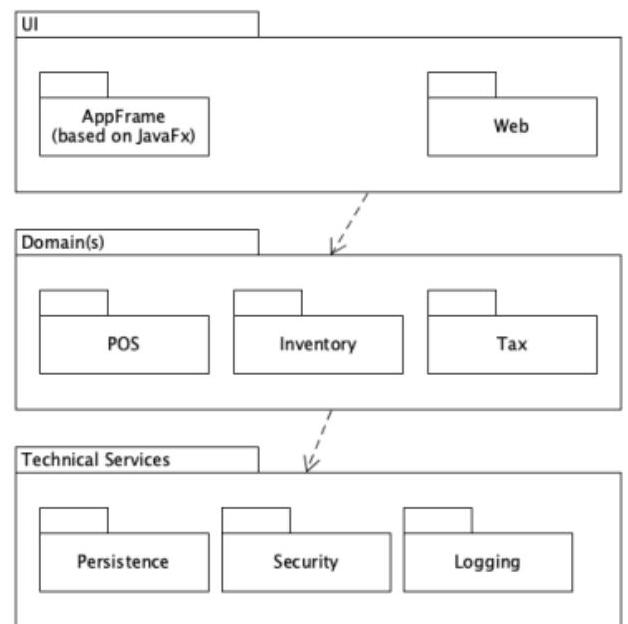
\includegraphics[width=0.9\linewidth]{images/2024_12_29_0d1d7b5551ea1b4b41bdg-09(1)}
\end{definition}

\begin{KR}{UML Diagrammauswahl}\\
Entscheidungshilfe für die Wahl des UML-Diagrammtyps:

\textbf{1. Strukturbeschreibung benötigt:}
\begin{itemize}
    \item Klassendiagramm für Typen und Beziehungen
    \item Paketdiagramm für Modularisierung
    \item Komponentendiagramm für Bausteinsicht
    \item Verteilungsdiagramm für Deployment
\end{itemize}

\textbf{2. Verhaltensbeschreibung benötigt:}
\begin{itemize}
    \item Sequenzdiagramm für Interaktionsabläufe
    \item Aktivitätsdiagramm für Workflows
    \item Zustandsdiagramm für Objektlebenszyklen
    \item Kommunikationsdiagramm für Objektkollaborationen
\end{itemize}

\textbf{3. Abstraktionsebene wählen:}
\begin{itemize}
    \item Analyse: Konzeptuelle Diagramme
    \item Design: Detaillierte Spezifikation
    \item Implementation: Codenahes Design
\end{itemize}
\end{KR}

\begin{concept}{Responsibility Driven Design (RDD)}\\
Design basierend auf Verantwortlichkeiten:
\begin{itemize}
    \item Klassenentwurf nach Rollen
    \item Kollaborationsbeziehungen
    \item Implementierung durch Attribute/Methoden
    \item Anwendbar auf allen Ebenen
\end{itemize}
\end{concept}

\begin{example2}{Prüfungsaufgabe: UML-Modellierung}
\textbf{Aufgabe:} 
Modellieren Sie für ein Bibliothekssystem die Ausleihe eines Buches mit:
\begin{itemize}
    \item Klassendiagramm der beteiligten Klassen
    \item Sequenzdiagramm des Ausleihvorgangs
    \item Zustandsdiagramm für ein Buchexemplar
\end{itemize}

\textbf{Bewertungskriterien:}
\begin{itemize}
    \item Korrekte UML-Notation
    \item Vollständigkeit der Modellierung
    \item Konsistenz zwischen Diagrammen
    \item Angemessener Detaillierungsgrad
\end{itemize}
%todo: add uml diagram
\end{example2}

\begin{theorem}{GRASP Prinzipien}\\
General Responsibility Assignment Software Patterns:
\begin{itemize}
    \item \textbf{Information Expert:} Verantwortung basierend auf Information
    \item \textbf{Creator:} Objekterstellung bei starker Beziehung
    \item \textbf{Controller:} Zentrale Steuerungslogik
    \item \textbf{Low Coupling:} Minimale Abhängigkeiten
    \item \textbf{High Cohesion:} Starker innerer Zusammenhang
    \item \textbf{Polymorphism:} Flexibilität durch Schnittstellen
    \item \textbf{Pure Fabrication:} Künstliche Klassen für besseres Design
    \item \textbf{Indirection:} Vermittler für Flexibilität
    \item \textbf{Protected Variations:} Kapselung von Änderungen
\end{itemize}
\end{theorem}

\begin{example2}{GRASP Anwendung}\\
\textbf{Szenario:} Online-Shop Warenkorb-Funktionalität

\textbf{GRASP-Prinzipien angewandt:}
\begin{itemize}
    \item \textbf{Information Expert:}
    \begin{itemize}
        \item Warenkorb kennt seine Positionen
        \item Berechnet selbst Gesamtsumme
    \end{itemize}
    
    \item \textbf{Creator:}
    \begin{itemize}
        \item Warenkorb erstellt Warenkorbpositionen
        \item Bestellung erstellt aus Warenkorb
    \end{itemize}
    
    \item \textbf{Controller:}
    \begin{itemize}
        \item ShoppingController koordiniert UI und Domain
        \item Keine Geschäftslogik im Controller
    \end{itemize}
    
    \item \textbf{Low Coupling:}
    \begin{itemize}
        \item UI kennt nur Controller
        \item Domain unabhängig von UI
    \end{itemize}
\end{itemize}
\end{example2}

\subsection{UML-Modellierung}

\begin{concept}{UML Diagrammtypen Übersicht}\\
UML bietet verschiedene Diagrammtypen für statische und dynamische Modellierung:

\textbf{Statische Modelle:}
\begin{itemize}
    \item Klassendiagramm
    \item Paketdiagramm
    \item Komponentendiagramm
    \item Verteilungsdiagramm
\end{itemize}

\textbf{Dynamische Modelle:}
\begin{itemize}
    \item Sequenzdiagramm
    \item Kommunikationsdiagramm
    \item Zustandsdiagramm
    \item Aktivitätsdiagramm
\end{itemize}
\end{concept}

\begin{definition}{Klassendiagramm}\\
\textbf{Hauptelemente:}
\begin{itemize}
    \item \textbf{Klassen:}
    \begin{itemize}
        \item Name der Klasse
        \item Attribute mit Sichtbarkeit
        \item Operationen mit Parametern
    \end{itemize}
    
    \item \textbf{Beziehungen:}
    \begin{itemize}
        \item Assoziation (normaler Pfeil)
        \item Vererbung (geschlossener Pfeil)
        \item Implementierung (gestrichelter Pfeil)
        \item Aggregation (leere Raute)
        \item Komposition (gefüllte Raute)
    \end{itemize}
    
    \item \textbf{Interfaces:}
    \begin{itemize}
        \item Stereotyp <<interface>>
        \item Nur Methodensignaturen
        \item Implementierungsbeziehung
    \end{itemize}
\end{itemize}
\end{definition}

\begin{example2}{Klassendiagramm: E-Commerce System}\\
\textbf{Domänenmodell mit wichtigen Beziehungen:}

\begin{lstlisting}[language=Java, style=basesmol]
public interface OrderRepository {
    Optional<Order> findById(OrderId id);
    void save(Order order);
}

public class Order {
    private OrderId id;
    private Customer customer;
    private List<OrderLine> orderLines;
    private OrderStatus status;
    
    public Money calculateTotal() {
        return orderLines.stream()
                        .map(OrderLine::getSubTotal)
                        .reduce(Money.ZERO, Money::add);
    }
}

public class OrderLine {
    private Product product;
    private int quantity;
    private Money price;
    
    public Money getSubTotal() {
        return price.multiply(quantity);
    }
}
\end{lstlisting}
\end{example2}

\begin{definition}{Sequenzdiagramm}\\
\textbf{Notationselemente:}
\begin{itemize}
    \item \textbf{Lebenslinien:}
    \begin{itemize}
        \item Objekte als Rechtecke
        \item Vertikale gestrichelte Linie
        \item Aktivierungsbalken für Ausführung
    \end{itemize}
    
    \item \textbf{Nachrichten:}
    \begin{itemize}
        \item Synchron (durchgezogener Pfeil)
        \item Asynchron (offener Pfeil)
        \item Antwort (gestrichelter Pfeil)
        \item Parameter und Rückgabewerte
    \end{itemize}
    
    \item \textbf{Kontrollelemente:}
    \begin{itemize}
        \item alt (Alternative)
        \item loop (Schleife)
        \item opt (Optional)
        \item par (Parallel)
    \end{itemize}
\end{itemize}
\end{definition}

\begin{example2}{Sequenzdiagramm: Bestellprozess}\\
\textbf{Interaktion zwischen Komponenten:}

\begin{lstlisting}[language=Java, style=basesmol]
public class OrderService {
    private final OrderRepository orderRepo;
    private final PaymentService paymentService;
    
    public OrderConfirmation processOrder(OrderRequest request) {
        // Validiere Bestellung
        validateOrder(request);
        
        // Erstelle Order
        Order order = createOrder(request);
        orderRepo.save(order);
        
        // Prozessiere Zahlung
        PaymentResult result = paymentService
            .processPayment(order.getId(), order.getTotal());
            
        // Bestaetige Bestellung
        if (result.isSuccessful()) {
            order.confirm();
            orderRepo.save(order);
            return new OrderConfirmation(order);
        }
        
        throw new PaymentFailedException();
    }
}
\end{lstlisting}
\end{example2}

\begin{definition}{Zustandsdiagramm}\\
\textbf{Notationselemente:}
\begin{itemize}
    \item \textbf{Zustände:}
    \begin{itemize}
        \item Startzustand (gefüllter Kreis)
        \item Endzustand (Kreis mit Punkt)
        \item Einfache Zustände (Rechteck)
        \item Zusammengesetzte Zustände
    \end{itemize}
    
    \item \textbf{Transitionen:}
    \begin{itemize}
        \item Event [Guard] / Action
        \item Interne Transitionen
        \item Selbsttransitionen
    \end{itemize}
    
    \item \textbf{Spezielle Elemente:}
    \begin{itemize}
        \item History State (H)
        \item Deep History (H*)
        \item Entry/Exit Points
        \item Choice Points
    \end{itemize}
\end{itemize}
\end{definition}

\begin{example2}{Zustandsdiagramm: Bestellstatus}\\
\textbf{Implementation eines State Patterns:}

\begin{lstlisting}[language=Java, style=basesmol]
public interface OrderState {
    void process(Order order);
    void cancel(Order order);
    void ship(Order order);
}

public class NewOrderState implements OrderState {
    @Override
    public void process(Order order) {
        validateOrder(order);
        order.setState(new ProcessingState());
    }
    
    @Override
    public void cancel(Order order) {
        order.setState(new CancelledState());
    }
    
    @Override
    public void ship(Order order) {
        throw new IllegalStateException(
            "Cannot ship new order");
    }
}

public class Order {
    private OrderState state;
    
    public void process() {
        state.process(this);
    }
    
    void setState(OrderState newState) {
        this.state = newState;
    }
}
\end{lstlisting}
\end{example2}

\begin{definition}{Aktivitätsdiagramm}\\
\textbf{Hauptelemente:}
\begin{itemize}
    \item \textbf{Aktionen:}
    \begin{itemize}
        \item Atomare Aktionen
        \item Call Behavior Action
        \item Send/Receive Signal
    \end{itemize}
    
    \item \textbf{Kontrollfluss:}
    \begin{itemize}
        \item Verzweigungen (Diamond)
        \item Parallelisierung (Balken)
        \item Join/Merge Nodes
    \end{itemize}
    
    \item \textbf{Strukturierung:}
    \begin{itemize}
        \item Activity Partitions (Swimlanes)
        \item Structured Activity Nodes
        \item Interruptible Regions
    \end{itemize}
\end{itemize}
\end{definition}

\begin{example2}{Aktivitätsdiagramm: Bestellabwicklung}\\
\textbf{Implementation eines Geschäftsprozesses:}

\begin{lstlisting}[language=Java, style=basesmol]
public class OrderProcessor {
    public void processOrder(Order order) {
        // Parallele Verarbeitung
        CompletableFuture.allOf(
            validateInventory(order),
            validatePayment(order)
        ).thenRun(() -> {
            if (order.isValid()) {
                fulfillOrder(order);
            } else {
                handleValidationFailure(order);
            }
        });
    }
    
    private CompletableFuture<Void> validateInventory(
            Order order) {
        return CompletableFuture.runAsync(() -> {
            order.getItems().forEach(item -> {
                if (!inventoryService.isAvailable(item)) {
                    throw new OutOfStockException(item);
                }
            });
        });
    }
}
\end{lstlisting}
\end{example2}

\begin{definition}{Verteilungsdiagramm}\\
\textbf{Elemente:}
\begin{itemize}
    \item \textbf{Nodes:}
    \begin{itemize}
        \item Device Nodes
        \item Execution Environment
        \item Artifacts
    \end{itemize}
    
    \item \textbf{Verbindungen:}
    \begin{itemize}
        \item Kommunikationspfade
        \item Protokolle
        \item Multiplizitäten
    \end{itemize}
    
    \item \textbf{Deployment:}
    \begin{itemize}
        \item Deployment Specifications
        \item Manifestationen
    \end{itemize}
\end{itemize}
\end{definition}

\begin{example2}{Verteilungsdiagramm: Microservice-Architektur}\\
\textbf{Deployment-Konfiguration:}

\begin{lstlisting}[language=Java, style=basesmol]
@Configuration
public class ServiceConfig {
    @Value("${service.host}")
    private String serviceHost;
    
    @Value("${service.port}")
    private int servicePort;
    
    @Bean
    public ServiceRegistry registry() {
        return ServiceRegistry.builder()
            .host(serviceHost)
            .port(servicePort)
            .healthCheck("/health")
            .build();
    }
    
    @Bean
    public LoadBalancer loadBalancer(
            ServiceRegistry registry) {
        return new RoundRobinLoadBalancer(registry);
    }
}
\end{lstlisting}
\end{example2}

\begin{definition}{Kommunikationsdiagramm}\\
\textbf{Hauptelemente:}
\begin{itemize}
    \item \textbf{Objekte:}
    \begin{itemize}
        \item Als Rechtecke dargestellt
        \item Mit Objektname und Klasse
        \item Verbunden durch Links
    \end{itemize}
    
    \item \textbf{Nachrichten:}
    \begin{itemize}
        \item Nummerierte Sequenz
        \item Synchrone/Asynchrone Aufrufe
        \item Parameter und Rückgabewerte
    \end{itemize}
    
    \item \textbf{Steuerungselemente:}
    \begin{itemize}
        \item Bedingte Nachrichten [condition]
        \item Iterationen *
        \item Parallele Ausführung || 
    \end{itemize}
\end{itemize}
\end{definition}

\begin{example2}{Kommunikationsdiagramm: Shopping Cart}\\
\textbf{Objektinteraktionen beim Checkout:}

\begin{lstlisting}[language=Java, style=basesmol]
public class ShoppingCart {
    private List<CartItem> items;
    private CheckoutService checkoutService;
    
    public Order checkout() {
        // 1: validateItems()
        validateItems();
        
        // 2: calculateTotal()
        Money total = calculateTotal();
        
        // 3: createOrder(items, total)
        Order order = checkoutService.createOrder(
            items, total);
            
        // 4: clearCart()
        items.clear();
        
        return order;
    }
}
\end{lstlisting}
\end{example2}

\begin{definition}{Paketdiagramm}\\
\textbf{Elemente:}
\begin{itemize}
    \item \textbf{Pakete:}
    \begin{itemize}
        \item Gruppierung von Modellelementen
        \item Hierarchische Strukturierung
        \item Namensräume
    \end{itemize}
    
    \item \textbf{Abhängigkeiten:}
    \begin{itemize}
        \item Import/Export von Elementen
        \item <<use>> Beziehungen
        \item Zugriffsrechte
    \end{itemize}
\end{itemize}
\end{definition}

\begin{KR}{UML Diagrammauswahl}\\
Entscheidungshilfen für die Wahl des passenden Diagrammtyps:

\textbf{1. Statische Struktur}
\begin{itemize}
    \item Klassendiagramm für Typen und Beziehungen
    \item Paketdiagramm für Modularisierung
    \item Komponentendiagramm für Bausteinsicht
    \item Verteilungsdiagramm für physische Verteilung
\end{itemize}

\textbf{2. Dynamisches Verhalten}
\begin{itemize}
    \item Sequenzdiagramm für zeitliche Abläufe
    \item Kommunikationsdiagramm für Objektkollaborationen
    \item Zustandsdiagramm für Objektlebenszyklen
    \item Aktivitätsdiagramm für Geschäftsprozesse
\end{itemize}

\textbf{3. Verwendungszweck}
\begin{itemize}
    \item Analyse: Konzeptuelle Modellierung
    \item Design: Detaillierte Spezifikation
    \item Implementation: Code-nahe Darstellung
    \item Dokumentation: Architekturübersicht
\end{itemize}
\end{KR}

\begin{example2}{UML in der Praxis}\\
\textbf{Beispiel eines kompletten Designs:}

\begin{lstlisting}[language=Java, style=basesmol]
// Paketstruktur
package com.example.shop;

// Domain Model
public class Product {
    private ProductId id;
    private String name;
    private Money price;
    private Category category;
}

// Service Layer
@Service
public class ProductService {
    private final ProductRepository repository;
    private final PriceCalculator calculator;
    
    public Product updatePrice(
            ProductId id, Money newPrice) {
        Product product = repository.findById(id)
            .orElseThrow(ProductNotFoundException::new);
            
        Money calculatedPrice = calculator
            .calculateFinalPrice(newPrice);
            
        product.updatePrice(calculatedPrice);
        return repository.save(product);
    }
}

// Controller Layer
@RestController
@RequestMapping("/api/products")
public class ProductController {
    private final ProductService service;
    
    @PutMapping("/{id}/price")
    public ProductDTO updatePrice(
            @PathVariable ProductId id,
            @RequestBody PriceUpdateRequest request) {
        Product product = service.updatePrice(
            id, request.getNewPrice());
        return ProductDTO.from(product);
    }
}
\end{lstlisting}
\end{example2}

